\documentclass{article}

\usepackage{graphicx}
\usepackage{tikz}
\usepackage{tikzsymbols}
\usetikzlibrary{calc,patterns,shapes.geometric}
\pagestyle{empty}
\usepackage[margin=0pt]{geometry}
\geometry{papersize={14in,12in}}

\def\centerarc[#1](#2)(#3:#4:#5){\draw[#1] ($(#2)+({#5*cos(#3)},{#5*sin(#3)})$) arc (#3:#4:#5);}

\begin{document}
	\begin{figure}
		\centering
		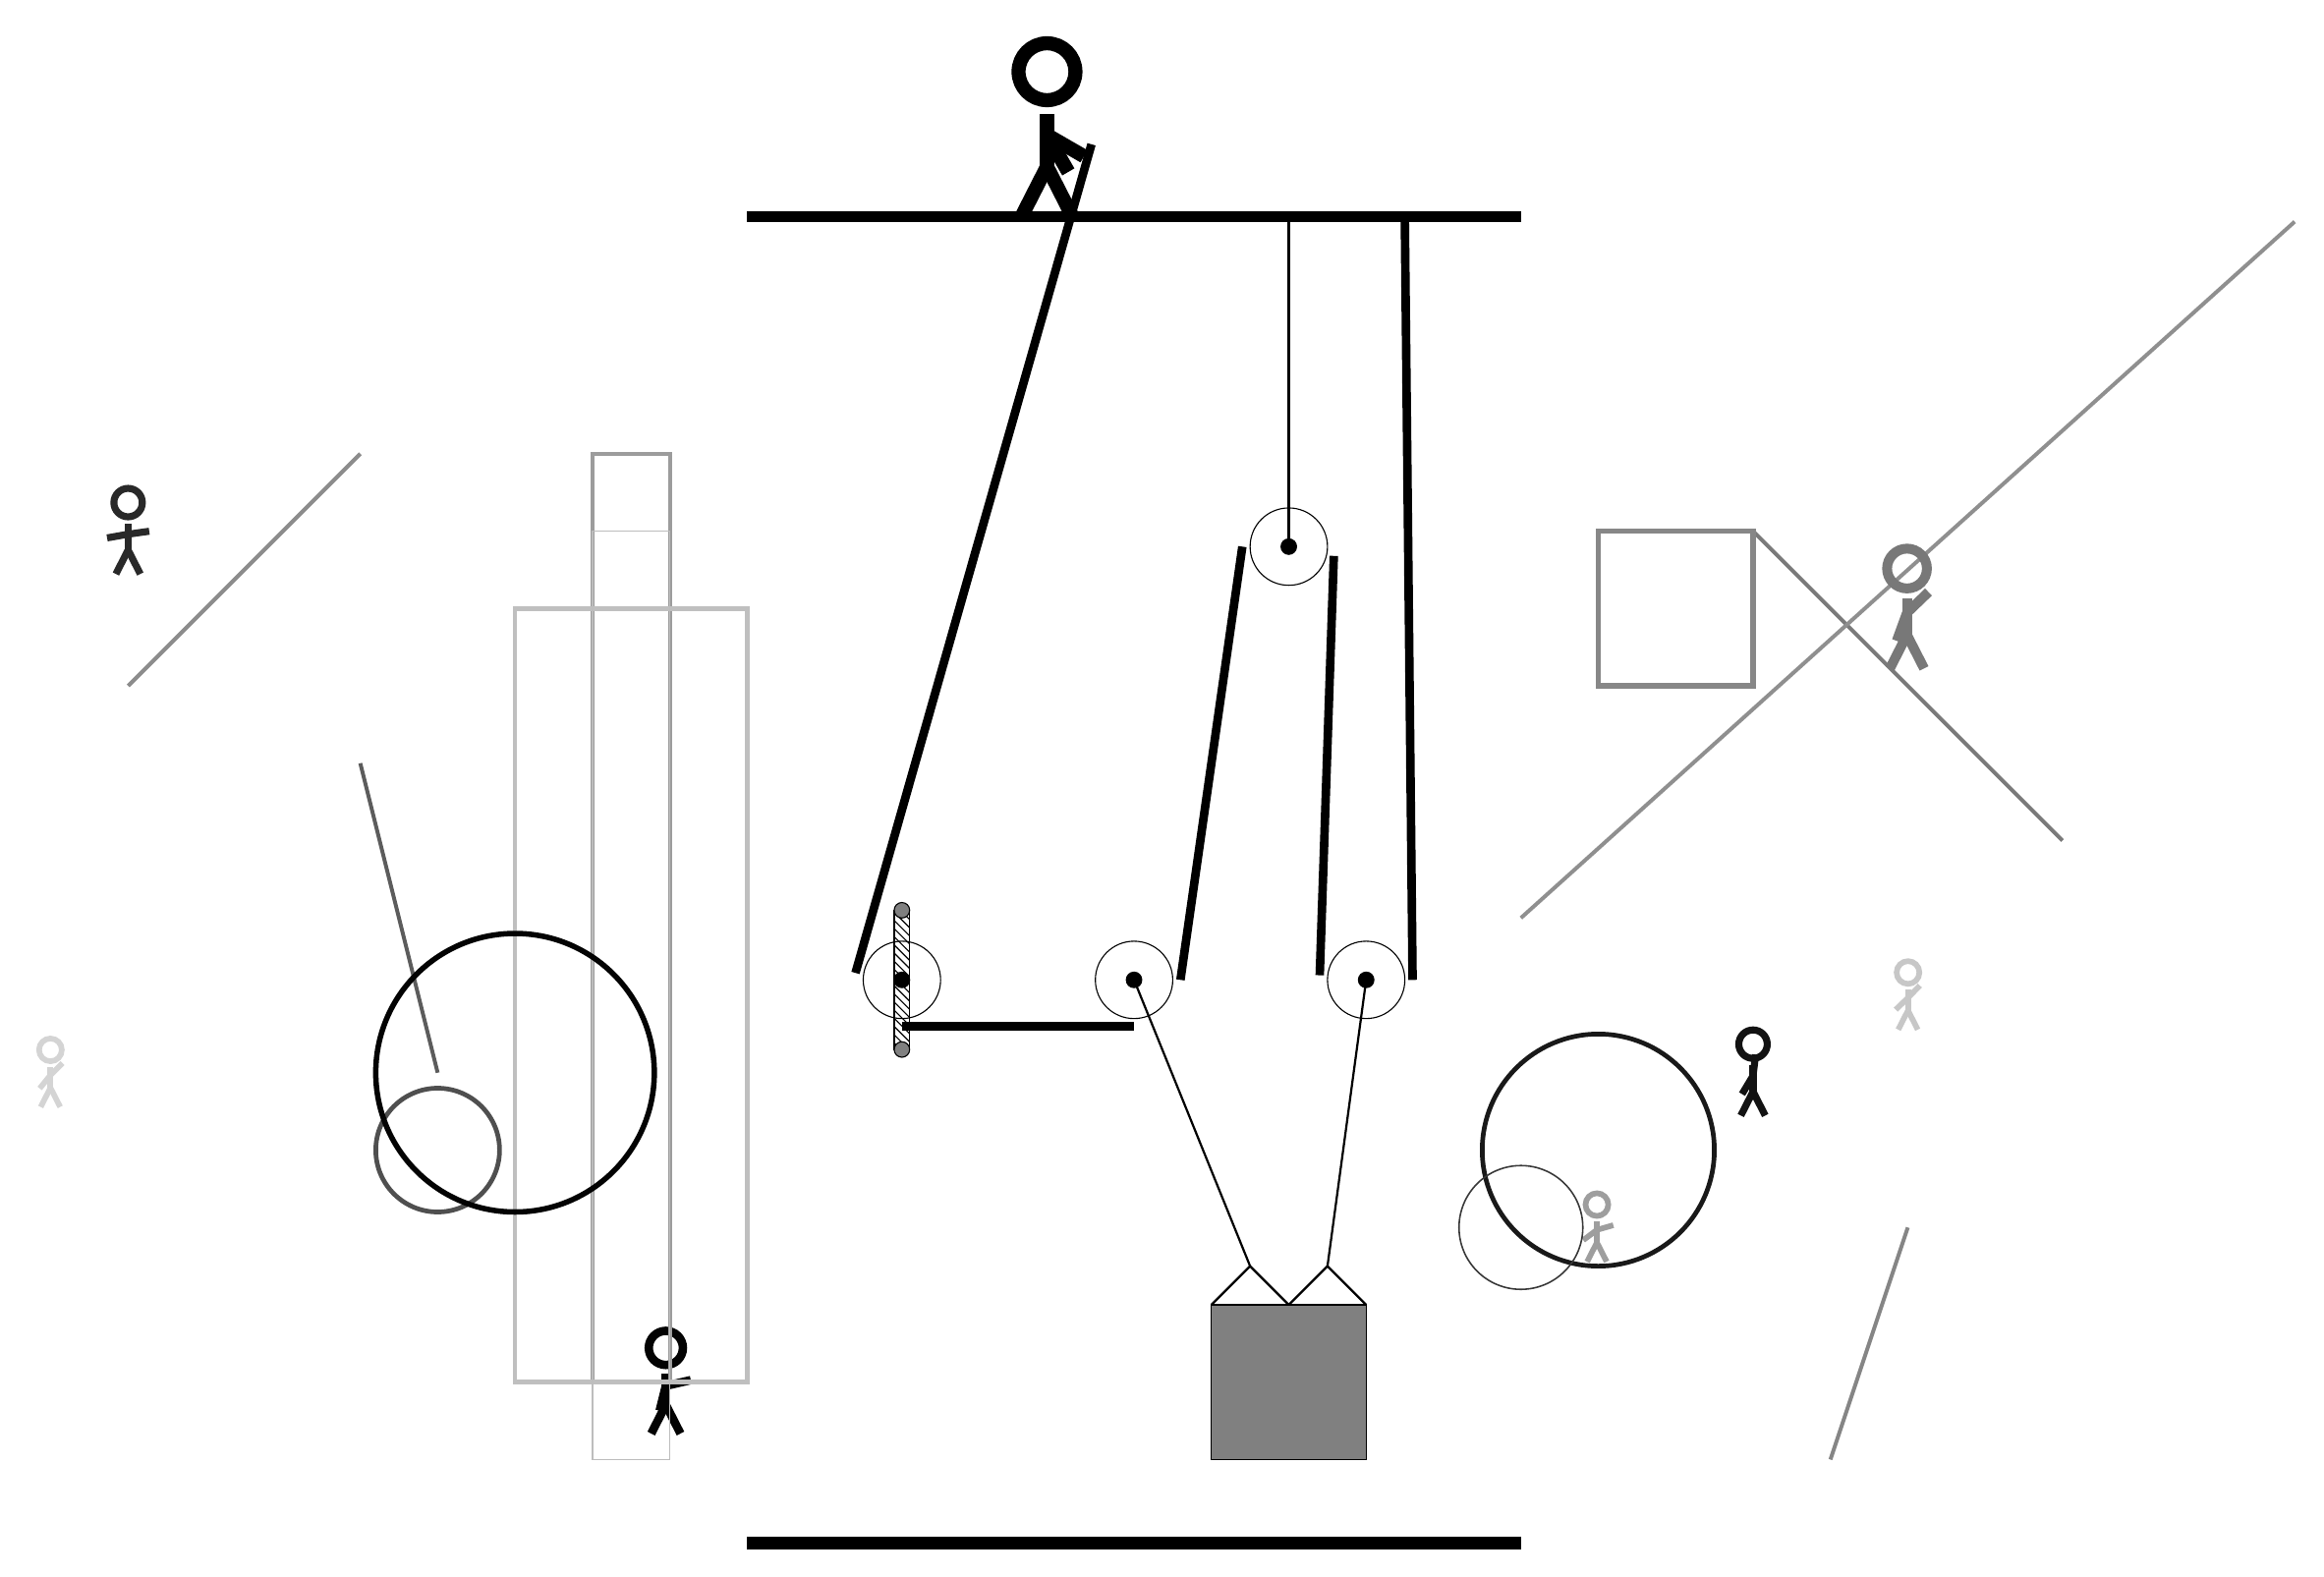
\begin{tikzpicture}
			%%%%% START %%%%%
			
			\draw[fill=black] (-4, 14) rectangle (6, 14.125);
			
			\draw (1, 4.2) circle (0.5);
			\draw[fill=black] (1, 4.2) circle (0.1);
			
			\draw (3, 9.8) circle (0.5);
			\draw[fill=black] (3, 9.8) circle (0.1);
			\draw[thick] (3, 9.8) -- (3, 14);
			
			\draw (4, 4.2) circle (0.5);
			\draw[fill=black] (4, 4.2) circle (0.1);
			
			\draw [line width=0.6mm, color=black!69](-8, 2) circle (0.8);
			
			\draw[line width=0.5mm, color=black!52](9, 10) -- (13, 6);
			\draw[line width=0.5mm, color=black!72] (-4, 3) rectangle (-4, 3);
			\node[line width=0.4mm, color=black!84] at (-12, 10) {\Strichmaxerl[5][10][8]};
			\node[line width=0.4mm, color=black!38] at (7, 1) {\Strichmaxerl[4][37][16]};
			\draw[line width=0.5mm, color=black!64](-9, 7) -- (-8, 3);
			
			\node[line width=0.5mm, color=black!17] at (-13, 3) {\Strichmaxerl[4][51][45]};
			\draw[line width=0.5mm, color=black!48](10, -2) -- (11, 1);
			\draw[line width=0.5mm, color=black!45](-9, 11) -- (-12, 8);
			
			\node[line width=0.6mm, color=black!99] at (-5, -1) {\Strichmaxerl[6][76][13]};
			\draw[line width=0.5mm, color=black!39] (-6, 11) rectangle (-5, -1);
			\draw[line width=0.6mm, color=black!25] (-4, 9) rectangle (-7, -1);
			\draw[line width=0.2mm, color=black!26] (-5, -2) rectangle (-6, 10);
			\draw [line width=0.7mm, color=black!99](-7, 3) circle (1.8);
			\draw[line width=0.7mm, color=black!47] (7, 8) rectangle (9, 10);
			\node[line width=0.3mm, color=black!93] at (9, 3) {\Strichmaxerl[5][59][83]};
			
			\draw[line width=0.5mm, color=black!44](6, 5) -- (16, 14);
			\node[line width=0.4mm, color=black!22] at (11, 4) {\Strichmaxerl[4][44][46]};
			\draw [line width=0.6mm, color=black!90](7, 2) circle (1.5);
			
			\draw [line width=0.2mm, color=black!78](6, 1) circle (0.8);
			\node[line width=0.7mm, color=black!53] at (11, 9) {\Strichmaxerl[7][70][44]};
			
			
			\draw[thick] (4, 4.2) -- (3.5, 0.5);
			\draw[thick] (1, 4.2) -- (2.5, 0.5);
			\draw[thick]  (2, 0) -- (2.5, 0.5) -- (3, 0);
			\draw[thick]  (3, 0) -- (3.5, 0.5) -- (4, 0);
			\draw[fill=black!50] (2, 0) rectangle (4, -2);
			
			\draw (-2, 4.2) circle (0.5);
			\draw[fill=black] (-2, 4.2) circle (0.1);
			\draw[pattern=north west lines, pattern color=black] (-2.1, 5.1) rectangle (-1.9, 3.3);
			\draw[fill=black!50] (-2, 5.1) circle (0.1);
			\draw[fill=black!50] (-2, 3.3) circle (0.1);
			
			\draw[line width=1.1mm] (0.45, 15) -- (-2.6, 4.29);
			\centerarc[line width=1.1mm](-2, 4.2)(160:270:0.6);
			\draw[line width=1.1mm](-2, 3.6) -- (1, 3.6);
			\centerarc[line width=1.1mm](1, 4.2)(270:360:0.6);
			\draw[line width=1.1mm] (1.6, 4.2) -- (2.4, 9.8);
			\centerarc[line width=1.1mm](3, 9.8)(-20:180:0.6);
			\draw[line width=1.1mm](3.582, 9.68) -- (3.4, 4.26);
			\centerarc[line width=1.1mm](4, 4.2)(160:360:0.6);
			\draw[line width=1.1mm](4.6, 4.2) -- (4.5, 14);
			
			\node at (-0.07, 15.2) {\Strichmaxerl[10][120][-30]};
			
			\draw[fill=black] (-4, -3) rectangle (6, -3.15);
			
			%%%%% END %%%%%
		\end{tikzpicture}
	\end{figure}	
\end{document}